\printconcepts

\exercise{A fundamental calculus technique is to use \underline{\hskip .5in} to refine approximations to get an exact answer.}{limits}

\exercise{What is the upper bound in the summation $\ds \sum_{i=7}^{14} (48i-201)$?}{14}

\exercise{This section approximates definite integrals using what geometric shape?}{Rectangles.}

\exercise{T/F: A sum using the Right Hand Rule is an example of a Riemann Sum.}{T}

\printproblems

\input{exercises/05_03_exset_01}

\begin{exerciseset}{In Exercises}{, write each sum in summation notation.}

\exercise{$3+6+9+12+15$}{Answers may vary; $\sum_{i=1}^5 3i$}

\exercise{$-1+0+3+8+15+24+35+48+63$}{Answers may vary; $\sum_{i=0}^8 (i^2-1)$}

\exercise{$\ds \frac12+\frac23+\frac34+\frac45$}{Answers may vary; $\sum_{i=1}^4 \frac{i}{i+1}$}

\exercise{$\ds 1-e+e^2-e^3+e^4$}{Answers may vary; $\sum_{i=0}^4 (-1)^ie^i$}

\end{exerciseset}


\exerciseset{In Exercises}{, evaluate the summation using \autoref{thm:summation}.}{

\exercise{$\ds \sum_{i=1}^{25} i$}{325}

\exercise{$\ds \sum_{i=1}^{10} (3i^2-2i)$}{1045}

\exercise{$\ds \sum_{i=1}^{15} (2i^3-10)$}{28,650}

\exercise{$\ds \sum_{i=1}^{10} (-4i^3+10i^2-7i+11)$}{$-8525$}

\exercise{$\ds \sum_{i=1}^{10} (i^3-3i^2+2i+7)$}{$2050$}

\exercise{$1+2+3+ \ldots + 99+100$}{$5050$}

\exercise{$1+4+9+ \ldots +361+400$}{$2870$}

}


\exerciseset{\autoref{thm:summation} states

$\ds \sum_{i=1}^na_i = \sum_{i=1}^k a_i + \sum_{i=k+1}^n a_i$\ , so 

$\ds \sum_{i=k+1}^na_i = \sum_{i=1}^n a_i - \sum_{i=1}^k a_i$\ .

\noindent Use this fact, along with other parts of \autoref{thm:summation}, to evaluate the summations given in Exercises}{.}{

\exercise{$\ds \sum_{i=11}^{20} i$}{$155$}

\exercise{$\ds \sum_{i=16}^{25} i^3$}{$91,225$}

\exercise{$\ds \sum_{i=7}^{12} 4$}{$24$}

\exercise{$\ds \sum_{i=5}^{10} 4i^3$}{$11,700$}

}


\ifthenelse{\boolean{printquestions}}{\columnbreak}{}

\input{exercises/05_03_exset_05}

\exerciseset{In Exercises}{, a definite integral $\ds \int_a^b f(x) \ dx$ is given. As demonstrated in Examples \ref{ex_rie9} and \ref{ex_rie10}, do the following.
\begin{enumerate}
\item[(a)]		Find a formula to approximate $\ds \int_a^bf(x)\ dx$ using $n$ subintervals and the provided rule.
\item[(b)]		Evaluate the formula using $n=10$, $100$ and $1,000$. 
\item[(c)]		Find the limit of the formula, as $n\to \infty$, to find the exact value of $\ds \int_a^bf(x)\ dx$.
\end{enumerate}
}{

\exercise{$\ds \int_{0}^1 x^3\ dx$, using the Right Hand Rule.
}{\begin{enumerate}
\item		Exact expressions will vary; $\frac{(1+n)^2}{4n^2}$.
\item		$121/400$, $10201/40000$, $1002001/4000000$
\item		$1/4$
\end{enumerate}
}

\exercise{$\ds \int_{-1}^1 3x^2\ dx$, using the Left Hand Rule.
}{\begin{enumerate}
\item		Exact expressions will vary; $2+4/n^2$.
\item		$51/25$, $5001/2500$, $500001/250000$
\item		$2$
\end{enumerate}
}

\exercise{$\ds \int_{-1}^3 (3x-1)\ dx$, using the Midpoint Rule.
}{\begin{enumerate}
\item		8.
\item		8, 8, 8
\item		$8$
\end{enumerate}
}

\exercise{$\ds \int_{1}^4 (2x^2-3)\ dx$, using the Left Hand Rule.
}{\begin{enumerate}
\item		Exact expressions will vary; $20/3-96/(3n)+64/(3n^2)$.
\item		$92/25$, $3968/625$, $103667/15625$
\item		$20/3$
\end{enumerate}
}

\exercise{$\ds \int_{-10}^{10} (5-x)\ dx$, using the Right Hand Rule.
}{\begin{enumerate}
\item		Exact expressions will vary; $100-200/n$.
\item		$80$, $98$, $499/5$
\item		$100$
\end{enumerate}
}

\exercise{$\ds \int_{0}^{1} (x^3-x^2)\ dx$, using the Right Hand Rule.
}{\begin{enumerate}
\item		Exact expressions will vary; $-1/12(1-1/n^2)$.
\item		$-33/400$, $-3333/40000$, $-333333/4000000$
\item		$-1/12$
\end{enumerate}
}
}

\ifthenelse{\boolean{printquestions}}{\columnbreak}{}

\exercise{Use six rectangles to approximate the area under the given graph of $f$ from $x=0$ to $x=12$, using:
\begin{enumerate}
\item The Left Hand Rule,
\item The Right Hand Rule,
\item The Midpoint Rule.
\end{enumerate}
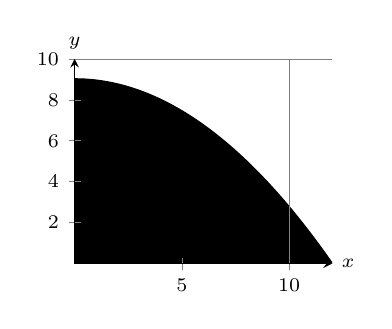
\begin{tikzpicture}
\begin{axis} [width=.4\textwidth,%\marginparwidth+25pt,
tick label style={font=\scriptsize},axis y line=middle,axis x line=middle,
name=myplot,axis on top,%all axes={grid},
                        ymin=0,ymax=10,
                        xmin=0,xmax=12,smooth]
   \addplot [{\coloronefill},fill={\coloronefill},area style,domain=0:12] {9-(x/4)^2} \closedcycle;
   \addplot [smooth,thick,{\colorone},domain=0:12] {9-(x/4)^2};
   \draw [help lines,step=10] (axis cs:0,0) grid (axis cs:12,10);
   % steps=10 was guess and check
\end{axis}
\node [right] at (myplot.right of origin) {\scriptsize $x$};
\node [above] at (myplot.above origin) {\scriptsize $y$};
\end{tikzpicture}}{\begin{enumerate}
\item	Exact expressions will vary; $80.5$.
\item	$72.25$
\item	$62.5$
\end{enumerate}}

\exercise{A car accelerates from 0 to 40 mph in 30 seconds. The speedometer reading at each 5 second interval during this time is given in the table below. Estimate how far the car travels during this 30 second period using the velocities at:
\begin{enumerate}
\item The beginning of each time interval.
\item The end of each time interval.
\end{enumerate}

\begin{center}
\begin{tabular} {|c|c|c|c|c|c|c|c|}
\hline
$\mathbf{t}$ (sec)&0&5&10&15&20&25&30\\ \hline
$\mathbf{v}$ (mph)&0&6&14&23&30&36&40\\ \hline
\end{tabular}
\end{center}}{\begin{enumerate}
\item	$(5\text{ s})((0+6+14+23+30+36)\text{ mph})=545\frac{\text{mi s}}{\text{hr}}\times\frac{1\text{ hr}}{3600\text{ s}}\times{5280\text{ ft}}{1\text{ mi}}=799\text{ ft}$
\item	$(5\text{ s})((6+14+23+30+36+40)\text{ mph})=585\frac{\text{mi s}}{\text{hr}}\times\frac{1\text{ hr}}{3600\text{ s}}\times{5280\text{ ft}}{1\text{ mi}}=858\text{ ft}$
\end{enumerate}}

\exercise{Use Theorems \ref{thm:summation} and \ref{thm:riemannSum} to justify the remaining property in Theorem \ref{thm:defintprop}: \[\int_a^b k\cdot f(x)\,dx =k\int_a^b f(x)\,dx\]}{\begin{align*}
\int_a^b k\cdot f(x)\,dx
&=\lim_{n\to\infty}\sum_{i=1}^n k\cdot f(c_i)\Delta x
\quad\text{T\ref{thm:riemannSum}.2} \\
&=\lim_{n\to\infty}k\cdot\sum_{i=1}^n k\cdot f(c_i)\Delta x
\quad\text{T\ref{thm:summation}.3} \\
&=k\cdot\lim_{n\to\infty}\sum_{i=1}^n k\cdot f(c_i)\Delta x
\quad\text{T\ref{thm:limit_algebra}.4} \\
&=k\int_a^b f(x)\,dx\quad\text{T\ref{thm:riemannSum}.2}
\end{align*}}

\exercise{Use Theorems \ref{thm:summation} and \ref{thm:riemannSum} to justify the remaining property in Theorem \ref{thm:further_def_int_props}: If $f(x)\leq M$ for all $x$ in $[a,b]$, then \[\int_a^b f(x)\,dx\leq M(b-a).\]}{Let $f$ and $M$ be as given.
\begin{align*}
\int_a^b f(x)\,dx
&=\lim_{n\to\infty}\sum_{i=1}^n f(c_i)\Delta x
\quad\text{T\ref{thm:riemannSum}.2} \\
&\le\lim_{n\to\infty}\sum_{i=1}^n M\Delta x \\
&=\int_a^b M\,dx\quad\text{T\ref{thm:riemannSum}.2} \\
&=M(b-a)
\end{align*}}

\printreview

\input{exercises/05_03_exset_07}
